\section{Методы нахождения оценок}

\subsection{Выборочные квантили}

\begin{note}
    Продолжим применять идею, что можно получать оценки параметра, если заменять характеристики истинной неизвестной функции распределения $F$ на характеристики эмпирической функции распределения $F_n^*$.
\end{note}

\begin{example}
    Пусть $F$ -- функция распределения, такая, что $F(0) = \frac{1}{2}$. Рассмотрим семейство распределений, отличающийся сдвигом, по-питоновски loc, $\{F(x-\theta),\ \theta \in \Theta\}$. Тогда в качестве оценки параметра $\theta$ разумно взять значение, относительно которого с меньшей и с большей стороны примерно одинаковое количество элементов выборки, например, такое: $\hat{\theta}_n(X) = X_{([\frac{n}{2}])}$.
\end{example}

\begin{definition}
    Пусть $P$ -- распределение вероятностей на $\R$, $F$ -- его функция распределения, $p \in (0, 1)$. $p$-квантилью распределения $P$ называют
    \[
        z_p = \inf \{x \in \R \colon F(x) \ge p\} = \min \{x \in \R \colon F(x) \ge p\}
    \]
    Инфимум достигается в силу того, что функция распределения непрерывна справа. При этом, если функция распределения имеет разрыв в точке $z_p$, то возможно, что $F(z_p) > p$.
\end{definition}

\begin{note}
    Если функция распределения $F$ непрерывна, то существует решение уравнения $F(x) = p$, не факт, что единственное. Если функция распределения $F$ монотонна, то решение уравнения $F(x) = p$ не более, чем единственно, правда, может не существовать.
\end{note}

\begin{definition}
    Пусть $X_1, \dots, X_n$ -- выборка. Выборочной $p$-квантилью называют статистику
    \[
        z_{n,p} = \System{
            & X_{(np)},\ np \in \Z,
            \\
            & X_{([np]+1)},\ np \notin \Z
        }
    \]
    Иными словами, берётся верхняя целая часть от $np$ и рассматривается порядковая статистика выборки с соответствующим номером.
\end{definition}

\begin{note}
    Выборочная $p$-квантиль $z_{n, p}$ из $X = (X_1, \dots, X_n)$ является $p$-квантилью эмпирической функции распределения $F_n^*$. Действительно, в силу того, что эмпирическая функция распределения строго возрастает лишь в точках выборки:
    \begin{multline*}
        \inf \{x \in \R \colon F_n^*(x) \ge p\} = \min \{X_k \in X \colon F_n^*(X_k) \ge p\} = \min \{X_{(k)} \in X \colon F_n^*(X_{(k)}) \ge p\} =
        \\
        = \min \set{X_{(k)} \in X \colon \frac{k}{n} \ge p} = \min \set{X_{(k)} \in X \colon k \ge np} = z_{n,p}
    \end{multline*}
\end{note}

\begin{note}
    И опять та же идея из метода подстановки, если умеем выражать параметр через квантиль распределения $\theta = G(P) = z_p$, то в качестве оценки этого параметра разумно взять аналог для эмпирической функции распределения $\hat{\theta} = G(P_n^*) = z_{n, p}$, то есть выборочную квантиль.
\end{note}

\begin{theorem} (О выборочной квантили)
    Пусть $X_1, \dots, X_n$ -- выборка из распределения $P$ с функцией распределения $F(x)$ и плотностью вероятности $f(x)$, то есть распределение абсолютно непрерывно. Пусть $z_p$ -- $p$-квантиль распределения $P$, причём $f$ непрерывно дифференцируема в окрестности точки $z_p$ и $f(z_p) > 0$. Тогда
    \[
        \sqrt{n}(z_{n,p} - z_p) \xrightarrow{d} N\ps{0, \frac{p(1-p)}{f^2(z_p)}}
    \]
\end{theorem}

\begin{proof}~
    \begin{itemize}
        \item Перепишем то, что хотим доказать, в более удобной эквивалентной форме:
        \begin{align*}
            & \sqrt{n}(z_{n,p} - z_p) \xrightarrow{d} \sqrt{\frac{p(1-p)}{f^2(z_p)}} N(0, 1)
            \\
            & \sqrt{\frac{n f^2(z_p)}{p(1-p)}}(z_{n,p} - z_p) \xrightarrow{d} N(0, 1)
        \end{align*}
        
        \item Идея доказательства состоит в следующем: сходимость по распределению $P_n \xrightarrow{d} P_0$ эквивалентна сходимости функций распределения $F_n$ к функции распределения $F_0$ в каждой точке непрерывности $F_0$, так как здесь $F_0$ относится к стандартному нормальному распределению, то просто в каждой точке. Но окажется, что здесь функции распределения устроены достаточно сложно, так что проще будет доказать сходимость плотностей, а потом из неё вывести сходимость функций распределения.

        \item Обозначим $k = \lceil np \rceil$, тогда $z_{n, p} = X_{(k)}$. Получим функцию распределения этой случайной величины:
        \[
            F_{X_{(k)}}(x) = P(X_{(k)} \le x) = \sum_{m=k}^n C_n^m F^m(x) (1-F(x))^{n-m}
        \]

        Поймём смысл того, что здесь написано. Вероятность того, что $X_{(k)} \le x$ является вероятностью того, что какие-то $m \ge k$ элементов выборки попали левее $x$. Сумма по $m$ позволяет зафиксировать, сколько элементов попало левее $x$, множитель $C_n^m$ фиксирует, какие именно элементы попали левее $x$, причём события
        \[
            \{X_{i_1} \le x, \dots, X_{i_m} \le x, X_{i_{m+1}} > x, \dots, X_{i_n} > x\}
        \]
        не пересекаются, поэтому вероятность их объединения распадается в сумму, и имеют вероятность $F^m(x) (1-F(x))^{n-m}$ в силу независимости элементов выборки и непрерывности функции распределения $F$.

        Так как последняя функция распределения абсолютна непрерывна, то она имеет плотность, которую можно получить дифференцированием:
        \begin{multline*}
            f_{X_{(k)}}(x) = F'_{X_{(k)}}(x) = \sum_{m=k}^n C_n^m [F^m(x) (1-F(x))^{n-m}]' =            \\
            = \sum_{m=k}^n C_n^m [F^m(x)]' (1-F(x))^{n-m} + \sum_{m=k}^n C_n^m F^m(x) [(1-F(x))^{n-m}]' =
            \\
            = \sum_{m=k}^n C_n^m m F^{m-1}(x) (1-F(x))^{n-m} f(x) + \sum_{m=k}^{n-1} C_n^m F^m(x) (n-m) (1-F(x))^{n-m-1} (-1) f(x)
        \end{multline*}

        Заметим, что во второй сумме после дифференцирования пропало последнее слагаемое, ибо производная от константы равна нулю. Теперь применим не очень хитрый трюк: $m C_n^m = m \frac{n!}{m!(n-m)!} = n \frac{(n-1)!}{(m-1)!(n-m)!} = n C_{n-1}^{m-1}$, $(n-m) C_n^m = n C_{n-1}^m$, тогда:
        \begin{multline*}
            f_{X_{(k)}} = \sum_{m=k}^n n C_{n-1}^{m-1} F^{m-1} (1-F)^{n-m} f + \sum_{m=k}^{n-1} n C_{n-1}^m F^m (1-F)^{n-m-1} (-1) f =
            \\
            = \sum_{m=k}^n n C_{n-1}^{m-1} F^{m-1} (1-F)^{n-m} f + \sum_{m=k+1}^{n} n C_{n-1}^{m-1} F^{m-1} (1-F)^{n-m} (-1) f =
            \\
            = n C_{n-1}^{m-1} F^{k-1} (1-F)^{n-k} f
        \end{multline*}

        Получили итоговую формулу для плотности случайной величины $X_{(k)}$:
        \[
            f_{X_{(k)}}(x) = n C_{n-1}^{k-1} F^{k-1}(x) (1-F(x))^{n-k} f(x)
        \]

        Теперь неформально поймём, почему эта формула естественна. Савёлов утверждал, что это рассуждение можно довести до формального, но я не умею это делать.
        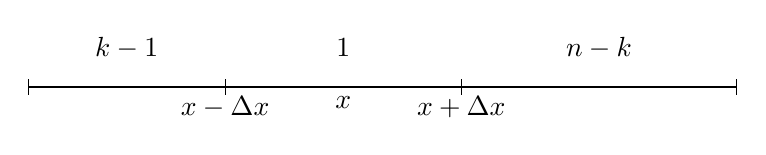
\begin{tikzpicture}
            \draw (0,0) -- (9,0);
            \draw (0,0.1) -- (0,-0.1);
            \draw (9,0.1) -- (9,-0.1);            
            
            \draw (2.5,0.1) -- (2.5,-0.1);
            \node at (2.5,0) [below] {$x - \Delta x$};
            \node at (4,0) [below] {$x$};
            \draw (5.5,0.1) -- (5.5,-0.1);
            \node at (5.5,0) [below] {$x + \Delta x$};
            
            \node at (1.25,0.5) {$k-1$};
            \node at (4,0.5) {$1$};
            \node at (7.25,0.5) {$n-k$};
        \end{tikzpicture}
        
        Учтём, что мы работаем с абсолютно непрерывными случайными величинами. Рассмотрим плотность случайной величины $X_{(k)}$ в точке $x$, возьмём малую окрестность $(x-\Delta x, x + \Delta x)$, тогда вероятность попадания $X_{(k)}$ в эту окрестность будет равна $f_{X_{(k)}}(x) \cdot 2\Delta x$. С другой стороны, эту же вероятность можно записать в другом виде: это вероятность того, что ровно $k-1$ точка попала левее и ровно $n-k$ точек попало правее. То есть сначала зафиксируем одну из $n$ точек, которая попадает в эту окрестность, $n$ вариантов, затем из оставшихся зафиксируем $k-1$ точку, попавшую левее, $C_{n-1}^{k-1}$ вариантов, после чего каждый такой исход будет иметь вероятность $F^{k-1}(x) \cdot f(x) \cdot 2\Delta x \cdot (1-F(x))^{n-k}$, по вероятностям попадания точек в левую, центральную и правую части соответственно.

        \item Вспомним, что по итогу хотим доказать:
        \[
            \sqrt{\frac{n f^2(z_p)}{p(1-p)}}(z_{n,p} - z_p) \xrightarrow{d} N(0, 1)
        \]

        Уже вводили обозначения $k = \lceil np \rceil$, $z_{n, p} = X_{(k)}$. Введём ещё: $C(n) = \sqrt{\frac{p(1-p)}{n f^2(z_p)}}$, и ещё: $\eta_n = \frac{1}{C(n)} (z_{n,p} - z_p)$, т.е. хотим доказать: $\eta_n \xrightarrow{d} N(0, 1)$. Распишем функцию распределения и плотность абсолютно непрерывной случайной величины $\eta_n$:
        \begin{multline*}
            F_{\eta_n}(x) = P(\eta_n \le x) = P\ps{\frac{1}{C(n)} (z_{n,p} - z_p) \le x} = P\ps{z_{n,p} \le z_p + C(n)x} =
            \\
            = P(X_{(k)} \le z_p + C(n)x) = F_{X_{(k)}}(z_p + C(n)x)
        \end{multline*}
        \[
            f_{\eta_n}(x) = F'_{\eta_n}(x) = (F_{X_{(k)}}(z_p + C(n)x))' = C(n) f_{X_{(k)}}(z_p + C(n)x)
        \]

        Теперь подставим полученную выше формулу для $f_{X_{(k)}}(x)$ и немного преобразуем результат, введя ещё обозначения $q = 1-p$ и $t(n, x) = z_p + C(n)x$:
        \begin{multline*}
            f_{\eta_n}(x) = C(n) f_{X_{(k)}}(t(n, x)) = C(n) n C_{n-1}^{k-1} [F(t(n, x))]^k [1-F(t(n, x))]^{n-k} f(t(n, x)) =
            \\
            = \sqrt{\frac{p(1-p)}{n f^2(z_p)}} n C_{n-1}^{k-1} [F(t(n, x))]^k [1-F(t(n, x))]^{n-k} f(t(n, x)) =
            \\
            = \sqrt{\frac{pq}{n f^2(z_p)}} n p^{k-1} q^{n-k} C_{n-1}^{k-1} \ps{\frac{F(t(n, x))}{p}}^k \ps{\frac{1-F(t(n, x))}{q}}^{n-k} f(t(n, x)) =
            \\
            = \sqrt{npq} C_{n-1}^{k-1} p^{k-1} q^{n-k} \cdot \frac{f(t(n, x))}{f(z_p)} \cdot \ps{\frac{F(t(n, x))}{p}}^k \ps{\frac{1-F(t(n, x))}{q}}^{n-k}
        \end{multline*}

        Специально подогнали формулу к последнему виду, чтобы было удобно разделить её на три части, и отдельно исследовать предел каждой из трёх частей:
        \begin{align*}
            & f_{\eta_n}(x) = A_1(n) \cdot A_2(n, x) \cdot A_3(n, x)
            \\
            & A_1(n) = \sqrt{npq} C_{n-1}^{k-1} p^{k-1} q^{n-k}
            \\
            & A_2(n, x) = \frac{f(t(n, x))}{f(z_p)}
            \\
            & A_3(n, x) = \ps{\frac{F(t(n, x))}{p}}^k \ps{\frac{1-F(t(n, x))}{q}}^{n-k}
        \end{align*}

        Теперь наш план состоит в следующем, докажем, что:
        \begin{align*}
            & A_1(n) \xrightarrow[n \to \infty]{} \frac{1}{\sqrt{2\pi}}
            \\
            & A_2(n, x) \xrightarrow[n \to \infty]{} 1
            \\
            & A_3(n, x) \xrightarrow[n \to \infty]{} e^{-\frac{x^2}{2}}
        \end{align*}

        Теперь поймём, что $f_{N(0,1)}(x) = \frac{1}{\sqrt{2\pi}} e^{-\frac{x^2}{2}}$ -- в точности плотность стандартного нормального распределения, то есть в таком случае докажем, что $f_{\eta_n}(x) \xrightarrow[n \to \infty]{} f_{N(0,1)}(x)$. С тем, как от этого перейти к сходимости для функций распределения, разберёмся позже, после того, как это докажем.

        \item $A_1(n) \xrightarrow[n \to \infty]{} \frac{1}{\sqrt{2\pi}}$. Утверждается, что здесь можно сослаться на результат из дискретного анализа, но так как я, во-первых, не помню этот результат и тем более его доказательство, во-вторых, видел не совсем аккуратные, а из-за этого совсем не корректные честные доказательства, проведём аккуратное рассуждение, посчитав предел. Воспользуемся только формулой Стирлинга $s! \sim \sqrt{2\pi s}\ps{\frac{s}{e}}^s$ и навыками из курса математического анализа.
        \begin{multline*}
            A_1(n) = \sqrt{npq} C_{n-1}^{k-1} p^{k-1} q^{n-k} = \sqrt{npq} p^{k-1} q^{n-k} \frac{(n-1)!}{(k-1)!(n-k)!} \sim
            \\
            \sim \sqrt{npq} p^{k-1} q^{n-k} \frac{\sqrt{\cancel{2\pi} (n-1)}\ps{\frac{n-1}{\cancel{e}}}^{n-1}}{\sqrt{\cancel{2\pi} (k-1)}\ps{\frac{k-1}{\cancel{e}}}^{k-1} \sqrt{2\pi (n-k)}\ps{\frac{n-k}{\cancel{e}}}^{n-k}} =
            \\
            = \frac{1}{\sqrt{2 \pi}} \frac{(n-1)^{n-1}}{(k-1)^{k-1} (n-k)^{n-k}} p^{k-1} q^{n-k} \sqrt{\frac{npq(n-1)}{(k-1)(n-k)}}
        \end{multline*}

        Теперь вспомним обозначения: $k = \lceil np \rceil$, $q = 1-p$, тогда $k \sim np$, $n-k \sim nq$, в таком случае получим:
        \[
            \sqrt{\frac{npq(n-1)}{(k-1)(n-k)}} \sim \sqrt{\frac{npq \cdot n}{np \cdot nq}} = 1
        \]

        То есть изначальное выражение можно переписать в следующем виде:
        \[
            A_1(n) \sim \frac{1}{\sqrt{2 \pi}} \frac{(n-1)^{n-1}}{(k-1)^{k-1} (n-k)^{n-k}} p^{k-1} q^{n-k} = \frac{1}{\sqrt{2 \pi}} \ps{\frac{(n-1)p}{k-1}}^{k-1} \ps{\frac{(n-1)q}{n-k}}^{n-k}
        \]

        Внутри каждой из двух последних скобок стоит выражение, эквивалентное 1, и оно возводится в степень, стремящуюся к бесконечности. Как знаем, такой предел может быть как $1$, так и, например, $e$, в формуле из его определения, так что просто заменить по эквивалентности не получится, и, как увидим из дальнейшего доказательства, сходимость здесь будет достаточно тонкой. Применим простое соображение: с пределом в произведении работать проще, чем с пределом в степени, поэтому перейдём к экспоненте и логарифмам:
        \[
            A_1(n) \sim \frac{1}{\sqrt{2 \pi}} \ps{\frac{(n-1)p}{k-1}}^{k-1} \ps{\frac{(n-1)q}{n-k}}^{n-k} = \frac{1}{\sqrt{2 \pi}} e^{(k-1) \ln\ps{\frac{(n-1)p}{k-1}} + (n-k) \ln\ps{\frac{(n-1)q}{n-k}}}
        \]

        Распишем то, как асимптотически устроены выражения из последней формулы, учитывая, что любое число отличается от своей целой части не более, чем на 1:
        \begin{align*}
            & k-1 = \lceil np \rceil - 1 = np - (np - \lceil np \rceil) - 1 = np + O(1)
            \\
            & n-k = n - \lceil np \rceil = nq + (np - \lceil np \rceil) = nq + O(1)
        \end{align*}    

        И, самое главное, логарифмы:
        \begin{multline*}
            \ln\ps{\frac{(n-1)p}{k-1}} = \ln\ps{\frac{np \ps{1 - \frac{1}{n}}}{np \ps{1 - \frac{np - \lceil np \rceil}{np} - \frac{1}{np}}}} =
            \\
            = \ln\ps{1 - \frac{1}{n}} - \ln\ps{1 - \frac{np - \lceil np \rceil}{np} - \frac{1}{np}} = - \frac{1}{n} + \frac{np - \lceil np \rceil}{np} + \frac{1}{np} + O\ps{\frac{1}{n^2}}
        \end{multline*}
        \begin{multline*}
            \ln\ps{\frac{(n-1)q}{n-k}} = \ln\ps{\frac{nq \ps{1 - \frac{1}{n}}}{nq \ps{1 + \frac{np - \lceil np \rceil}{nq}}}} =
            \\
            = \ln\ps{1 - \frac{1}{n}} - \ln\ps{1 + \frac{np - \lceil np \rceil}{nq}} = - \frac{1}{n} - \frac{np - \lceil np \rceil}{nq} + O\ps{\frac{1}{n^2}}
        \end{multline*}

        Теперь заметим, что множитель перед логарифмом имеет порядок $n$, а сам логарифм имеет порядок $\frac{1}{n}$, поэтому то, что было вынесено в $O$-большие, в пределе уйдёт в ноль и не будет иметь значения, тогда имеем переход:
        \begin{multline*}
            A_1(n) \sim \frac{1}{\sqrt{2\pi}} e^{np\ps{- \frac{1}{n} + \frac{np - \lceil np \rceil}{np} + \frac{1}{np}} + nq\ps{- \frac{1}{n} - \frac{np - \lceil np \rceil}{nq}}} =
            \\
            = \frac{1}{\sqrt{2\pi}} e^{-p + np - \lceil np \rceil + 1 - q - np + \lceil np \rceil} = \frac{1}{\sqrt{2\pi}} e^{-p + 1 - q} = \frac{1}{\sqrt{2\pi}}
        \end{multline*}

        \item $A_2(n, x) = \frac{f(t(n, x))}{f(z_p)} \xrightarrow[n \to \infty]{} 1$. Так же, как долго мы расправлялись с предыдущим пределом, быстро справимся с этим. Действительно, раскроем обозначения:
        \[
            t(n, x) = z_p + C(n)x = z_p + \frac{1}{\sqrt{n}} \sqrt{\frac{p(1-p)}{f^2(z_p)}} x \xrightarrow[n \to \infty]{} z_p
        \]

        В силу непрерывности, и даже непрерывной дифференцируемости, функции плотности $f(x)$, числитель $f(t(n, x))$ дроби $A_2(n, x)$ сходится к знаменателю $f(z_p)$, в силу чего вся дробь $A_2(n, x)$ сходится к единице.

        \item $A_3(n, x) \xrightarrow[n \to \infty]{} e^{-\frac{x^2}{2}}$. Здесь будет проще доказать в эквивалентном виде:
        \[
            \ln A_3(n, x) = k \ln \ps{\frac{F(t(n, x))}{p}} + (n-k) \ln \ps{\frac{1-F(t(n, x))}{q}} \xrightarrow[n \to \infty]{} -\frac{x^2}{2}
        \]

        Уже выяснили, что $t(n, x)$ стремится к $z_p$, то есть находится в малой окрестности точки $z_p$. Применим, в связи с этим, разложение по формуле Тейлора до второго порядка функции $F$, которая дважды непрерывно дифференцируема, в силу того, что $f = F'$ непрерывно дифференцируема.
        \[
            F(t(n, x)) = F(z_p) + (t(n, x) - z_p) F'(z_p) + \frac{1}{2} (t(n, x) - z_p)^2 F''(z_p) + O(|t(n, x) - z_p|^3)
        \]

        В силу обозначений $t(n, x) - z_p = C(n) x = \sqrt{\frac{p(1-p)}{n f^2(z_p)}} x$. В силу того, что $z_p$ -- $p$-квантиль, $F(z_p) = p$, в силу того, что плотность -- производная функции распределения, получим $F'(z_p) = f(z_p)$, $F''(z_p) = f'(z_p)$, также $q = 1-p$. Тогда перепишем разложение по формуле Тейлора:
        \begin{multline*}
            F(t(n, x)) = p + \sqrt{\frac{p(1-p)}{n f^2(z_p)}} x f(z_p) + \frac{1}{2} \frac{p(1-p)}{n f^2(z_p)} x^2 f'(z_p) + O\ps{\frac{1}{n \sqrt{n}}} =
            \\
            = p + \sqrt{\frac{pq}{n}} x + \frac{1}{2} \frac{pq}{n} x^2 \frac{f'(z_p)}{f^2(z_p)} + O\ps{\frac{1}{n \sqrt{n}}}
        \end{multline*}

        Введём фундаментальную константу $\alpha = \frac{1}{2} \frac{f'(z_p)}{f^2(z_p)} pq$, ещё раз вспомним, что $p = 1-q$, получим:
        \begin{align*}
            & \frac{F(t(n, x))}{p} = 1 + \frac{1}{p} \sqrt{\frac{pq}{n}} x + \frac{1}{p} \frac{\alpha x^2}{n} + O\ps{\frac{1}{n \sqrt{n}}}
            \\
            & \frac{1-F(t(n, x))}{q} = 1 - \frac{1}{q} \sqrt{\frac{pq}{n}} x - \frac{1}{q} \frac{\alpha x^2}{n} + O\ps{\frac{1}{n \sqrt{n}}}
        \end{align*}

        Теперь разложим по формуле Тейлора логарифмы последних выражений, первого порядка не хватит, придётся залезть в квадраты:
        \begin{align*}
            & \ln \ps{\frac{F(t(n, x))}{p}} = \frac{1}{p} \sqrt{\frac{pq}{n}} x + \frac{1}{p} \frac{\alpha x^2}{n} + O\ps{\frac{1}{n \sqrt{n}}} - \frac{1}{2} \ps{\frac{1}{p} \sqrt{\frac{pq}{n}} x}^2 + O\ps{\frac{1}{n \sqrt{n}}}
            \\
            & \ln\ps{\frac{1-F(t(n, x))}{q}} = -\frac{1}{q} \sqrt{\frac{pq}{n}} x - \frac{1}{q} \frac{\alpha x^2}{n} + O\ps{\frac{1}{n \sqrt{n}}} - \frac{1}{2} \ps{-\frac{1}{q} \sqrt{\frac{pq}{n}} x}^2 + O\ps{\frac{1}{n \sqrt{n}}}
        \end{align*}

        Ещё немного упростив, получим:
        \begin{align*}
            & \ln \ps{\frac{F(t(n, x))}{p}} = \frac{1}{p} \sqrt{\frac{pq}{n}} x + \frac{1}{p} \frac{\alpha x^2}{n} - \frac{1}{2} \frac{q}{np} x^2 + O\ps{\frac{1}{n \sqrt{n}}}
            \\
            & \ln\ps{\frac{1-F(t(n, x))}{q}} = -\frac{1}{q} \sqrt{\frac{pq}{n}} x - \frac{1}{q} \frac{\alpha x^2}{n} - \frac{1}{2} \frac{p}{nq} x^2 + O\ps{\frac{1}{n \sqrt{n}}}
        \end{align*}

        Вспомним формулы, которые получали ранее: $k-1 = np + O(1)$, $n-k = nq + O(1)$. В силу порядков множителей перед логарифмами и логарифмов в $\ln A_3(n, x)$, слагаемые с $O$-большим вновь никак не будут влиять на предел, тогда:
        \begin{multline*}
            \ln A_3(n, x) = k \ln \ps{\frac{F(t(n, x))}{p}} + (n-k) \ln \ps{\frac{1-F(t(n, x))}{q}} =
            \\
            = np \ps{\cancel{\frac{1}{p} \sqrt{\frac{pq}{n}} x} + \cancel{\frac{1}{p} \frac{\alpha x^2}{n}} - \frac{1}{2} \frac{q}{np} x^2} + nq \ps{\cancel{-\frac{1}{q} \sqrt{\frac{pq}{n}} x} - \cancel{\frac{1}{q} \frac{\alpha x^2}{n}} - \frac{1}{2} \frac{p}{nq} x^2} + o(1) =
            \\
            = -\frac{1}{2} qx^2 -\frac{1}{2} px^2 + o(1) = -\frac{1}{2} x^2 + o(1)
        \end{multline*}

        \item Теперь, пока ещё не прошла радость от того, что все пределы наконец-то сошлись, узнаем ещё одну вещь. Мы доказали сходимость плотностей $f_{\eta_n}(x) \xrightarrow[n \to \infty]{} f_{N(0, 1)}(x)$ поточечно по $x$. Нам же понадобится сходимость чуть сильнее: равномерно на каждом отрезке $[-N, N]$. Что же, пойдём расписывать заново все пределы и проверять равномерную сходимость (нет). Формально расписывать это не будем, но понять, почему именно на отрезках и почему сходимость равномерная, не слишком сложно. Где вообще у нас появлялись сходимости, а не арифметические равенства -- в $O$-больших, именно они отвечали за то, что уходило в ноль при $n \to \infty$, всё остальное сокращалось арифметически. Как при сходимостях у нас участвовал $x$ -- только в $A_2(n, x)$ и $A_3(n, x)$, вылезал как $x^s$ для некоторого $s$. На отрезке $[-N, N]$ можно мажорировать $|x^s| = |x|^s \le N^s$ и сохранить полученную сходимость, точнее, сделать её равномерной. И по-хорошему, чтобы написать формулу Тейлора с остаточным членом в форме Лагранжа, нам достаточно просто дифференцируемости $f$, а для того, чтобы оценить его константой, для $O$-большого, мы как раз и используем непрерывную дифференцируемость $f$.

        \item Итак, знаем на текущий момент: $f_{\eta_n}(x) \xrightarrow[n \to \infty]{} f_{N(0, 1)}(x)$ равномерно на любом компакте $[-N, N]$. Хотим отсюда получить поточечную сходимость функций распределения $F_{\eta_n}(x) \xrightarrow[n \to \infty]{} F_{N(0, 1)}(x)$, тогда теорема будет доказана. Идейно понятно, что хочется сделать: взять большой компакт, что на хвостах плотности $f_{\eta_n}$ и $f_{N(0, 1)}$ будут малы, а на компакте устремить $n \to \infty$, тогда функции распределения, как интегралы от плотностей, тоже будут слабо отличаться. Вопрос лишь, как аккуратно выбрать компакт, чтобы выбор не зависел от $n$, то есть чтобы устремление $n \to \infty$ было корректным. Оказывается, что компакт можно выбрать лишь по плотности предела, то есть $f_{N(0, 1)}$.

        Подбёрем $N$ так, что плотность $N(0, 1)$ на хвостах мала:
        \[
            \lim_{N \to \infty} \int_{[-N, N]} f_{N(0, 1)}(x) d\mu(x) = 1 \Ra \exists N \ \int_{\R \setminus [-N, N]} f_{N(0, 1)}(x) d\mu(x) < \eps
        \]

        Тогда можем оценить и плотности на хвостах $\eta_n$:
        \begin{multline*}
            \int_{\R \setminus [-N, N]} f_{\eta_n}(x) d\mu(x) = \md{\int_{\R \setminus [-N, N]} f_{\eta_n}(x) d\mu(x)} =
            \\
            = \md{\int_{\R \setminus [-N, N]} f_{N(0, 1)}(x) d\mu(x) - \int_{\R \setminus [-N, N]} f_{N(0, 1)}(x) d\mu(x) + \int_{\R \setminus [-N, N]} f_{\eta_n}(x) d\mu(x)} =
            \\
            = \md{\int_{\R \setminus [-N, N]} f_{N(0, 1)}(x) d\mu(x) - \cancel{1} + \int_{[-N, N]} f_{N(0, 1)}(x) d\mu(x) + \cancel{1} - \int_{[-N, N]} f_{\eta_n}(x) d\mu(x)} \le
            \\
            \le \int_{\R \setminus [-N, N]} f_{N(0, 1)}(x) d\mu(x) + \int_{[-N, N]} |f_{\eta_n}(x) - f_{N(0, 1)}(x)| d\mu(x)
        \end{multline*}

        Здесь первый интеграл меньше $\eps$ по выбору $N$, для второго возьмём $n$ настолько большим, что равномерно $|f_{\eta_n}(x) - f_{N(0, 1)}(x)| < \frac{\eps}{2N}$, можем так сделать, потому что компакт, тогда:
        \[
            \int_{\R \setminus [-N, N]} f_{\eta_n}(x) d\mu(x) \le \eps + \frac{\eps}{2N} \cdot 2N = 2 \eps
        \]

        Тогда оценим разность функций распределения в какой-то конкретной точке:
        \begin{multline*}
            | F_{\eta_n}(x) - F_{N(0, 1)}(x) | = \md{\int_{(-\infty, x]} f_{\eta_n}(x) d\mu(x) - \int_{(-\infty, x]} f_{N(0, 1)}(x) d\mu(x)} \le
            \\
            \le \int_{(-\infty, -N]} f_{\eta_n}(x) d\mu(x) + \int_{(-\infty, -N]} f_{N(0, 1)}(x) d\mu(x) + \int_{[-N, x]} |f_{\eta_n}(x) - f_{N(0, 1)}(x)| d\mu(x)
        \end{multline*}

        Выберем $n$ ещё больше, чтобы на компакте $[-N, x]$ интеграл тоже был меньше $\eps$, получим:
        \[
            | F_{\eta_n}(x) - F_{N(0, 1)}(x) | \le 2 \eps + \eps + \eps = 4 \eps
        \]
    \end{itemize}
\end{proof}

\begin{note}
    Медианой называют $1/2$-квантиль $z_{1/2}$. Выборочную медиану определим немного иначе, чем выборочную квантиль, но сути это не поменяет.
\end{note}

\begin{definition}
    Пусть $X_1, \dots, X_n$ -- выборка. Выборочной медианой называют статистику
    \[
        \hat{\mu} = \System{
            & X_{(k)},\ n = 2k+1,
            \\
            & \frac{X_{(k)} + X_{(k+1)}}{2},\ n = 2k
        }
    \]
\end{definition}

\begin{theorem} (О выборочной медиане, б/д)
    Пусть $X_1, \dots, X_n$ -- выборка из распределения $P$ с функцией распределения $F(x)$ и плотностью вероятности $f(x)$, то есть распределение абсолютно непрерывно. Пусть $z_{1/2}$ -- $1/2$-квантиль распределения $P$, причём $f$ непрерывно дифференцируема в окрестности точки $z_{1/2}$ и $f(z_{1/2}) > 0$. Тогда
    \[
        \sqrt{n}(\hat{\mu} - z_{1/2}) \xrightarrow{d} N\ps{0, \frac{1}{4 f^2(z_{1/2})}}
    \]
\end{theorem}